\begin{enumerate}
	\item L'administrateur se rend sur le panel admin. 
	\item Il sélectionne \textit{Etats Abonnement} dans le menu. 
	\item L'administrateur atterris sur la page de gestion des abonnement 
	\item Il clique sur \textit{Renouveler} pour relancer l'abonnement d'un utilisateurs. 
\end{enumerate}

\begin{figure}[h]
	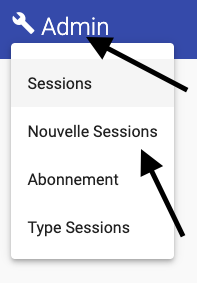
\includegraphics[width=0.4\textwidth,center]{Figures/us11-1}
	\caption{Bouton Etats Abonnement}
\end{figure}

\vspace{\baselineskip}
\vspace{\baselineskip}
\begin{figure}[h]
	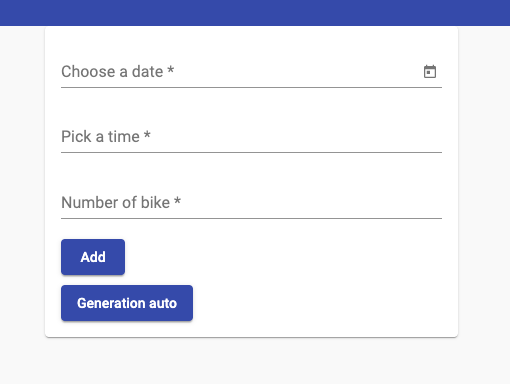
\includegraphics[width=0.5\textwidth,center]{Figures/us11-2}
	\caption{Bouton de renouvellement de l'abonnement}
\end{figure}

\vspace{\baselineskip}
\subsubsection{Script concerné}
	\begin{itemize}
		\item \Href{https://github.com/victorsmits/Aquabike/blob/master/Symfony-Twig/src/Entity/Person.php}{Person.php}
		\item \Href{https://github.com/victorsmits/Aquabike/blob/master/Symfony-Twig/src/Controller/AbonnementController.php}{AbonnementController.php}
		\item \Href{https://github.com/victorsmits/Aquabike/blob/master/Symfony-Twig/templates/create_session/abonnement.html.twig}{abonnement.html.twig}
	\end{itemize}